\documentclass[conference]{IEEEtran}
\IEEEoverridecommandlockouts

\usepackage{amsmath,amssymb}
\usepackage{graphicx}
\usepackage{booktabs}
\usepackage{multirow}
\usepackage{xcolor}
\usepackage{tikz}
\usetikzlibrary{arrows.meta,positioning,fit,backgrounds}
\usepackage[hidelinks]{hyperref}
\usepackage{url}
\usepackage{cite}

\graphicspath{{../figures/}{figures/}} % repo layout, or flat Overleaf upload
% Values still to be measured in the v2 Colab run, or links still to be added.
\newcommand{\tbd}[1]{\textcolor{red}{\textbf{#1}}}

% Two-column floats: allow two full-width figures at a page top and fuller float pages,
% so the Section IV figures don't pile up at the end of the paper.
\renewcommand{\topfraction}{0.9}
\renewcommand{\dbltopfraction}{0.9}
\renewcommand{\textfraction}{0.07}
\renewcommand{\floatpagefraction}{0.8}
\renewcommand{\dblfloatpagefraction}{0.8}
\setcounter{topnumber}{3}
\setcounter{dbltopnumber}{2}
\setcounter{totalnumber}{4}

\begin{document}

\title{History Overrides Perception: Hallucinated Belief Persistence\\in Vision-Language Models for Sequential Driving Perception}

\author{
\IEEEauthorblockN{Nickzad Bayati and Toney Zhen}
\IEEEauthorblockA{Department of Computer Engineering, San Jos\'e State University\\
Code: \url{https://github.com/n-zad/av-vlm-belief-persistence}\quad
Video demo: \tbd{[add link]}}
}

\maketitle

\begin{abstract}
Vision-language models (VLMs) are increasingly proposed as perception components for autonomous vehicles, where they are queried repeatedly over a stream of camera frames. We ask whether a VLM that reported no pedestrian while the pedestrian was mostly occluded keeps that answer after the pedestrian becomes clearly visible. We mine 145 six-frame nuScenes front-camera sequences in which a pedestrian goes from 0--40\% to 80--100\% visible, and query Qwen2.5-VL-7B and LLaVA-OneVision-7B on every frame without history (stateless), with the conversation history (stateful), and with history plus an instruction to reconsider. The first frame is identical across modes and produced identical answers in all 145 sequences for both models, so the history is the only difference. History lowers post-evidence accuracy by 25 points (95\% CI 19--32) for Qwen and 22 points (14--30) for LLaVA; on evidence frames each model detects without history, it still detects only 21\% and 60\% with history. The mechanism is answer copying: with history, 78\% and 93\% of answers repeat the previous one verbatim. Reconsidering does not help; only resetting the history does. A fixed wrong ``no'' planted in the history has the same effect (21\% and 43\% still detected), and on 75 pedestrian-free control sequences a planted wrong ``yes'' persists too: LLaVA repeats it on every frame, and Qwen on 95\% of empty frames after four planted turns. The failure is therefore generic answer copying rather than a belief specific to absence. We release the full pipeline.
\end{abstract}

\begin{IEEEkeywords}
vision-language models, hallucination, autonomous driving, temporal consistency, evaluation
\end{IEEEkeywords}

% ---------------------------------------------------------------------------
\section{Introduction}

Vision-language models are being integrated into autonomous-driving stacks as scene describers, question answerers and driving assistants~\cite{guo2024vlmauto,xie2025drivebench,lin2025continual}. In deployment such a model does not see one image: it is queried every few hundred milliseconds, and the simplest way to give it context is to keep the conversation, so that each new frame arrives together with the model's earlier frames and answers.

This creates a safety risk that single-image benchmarks cannot expose. If the model wrongly reports that no pedestrian is present while the pedestrian is occluded, its own ``no'' becomes part of the context for every later frame. When the pedestrian then steps into full view, the model may defer to its earlier answer instead of the new image. In driving, that is a missed pedestrian at exactly the moment the evidence is clearest.

Measuring this effect is hard for four reasons. First, it needs sequences with temporal ground truth in which the evidence changes from ambiguous to clear. Second, a wrong answer on a clear frame can come from poor perception rather than from the history, so the two must be separated. Third, the comparison must hold everything except the history fixed. Fourth, a ``no'' on an occluded frame is often a reasonable call rather than a hallucination, so a study built only on the model's own errors cannot tell how strongly a wrong belief is held. Existing work evaluates VLMs on single frames, on corrupted inputs~\cite{xie2025drivebench}, or on the consistency of repeated answers~\cite{chang2026futurevqa}, and object-hallucination benchmarks~\cite{li2023pope,rohrbach2018chair} use single images.

We address these with a controlled stateful-versus-stateless protocol on nuScenes~\cite{caesar2020nuscenes}. Our contributions are:
\begin{itemize}
  \item A \textbf{sequence-mining procedure} that extracts 145 front-camera sequences in which a pedestrian goes from at most 40\% to at least 80\% visible, using only the nuScenes metadata and camera geometry.
  \item A \textbf{controlled protocol} that runs each sequence statelessly, statefully and with a reconsider instruction, verified to differ only in the history (identical frame-0 answers in 145/145 sequences for both models).
  \item A \textbf{planted-belief experiment} that writes a fixed wrong answer into the history before the evidence frame, so the belief is not one the model formed itself, and measures how much evidence it takes to overturn it.
  \item \textbf{Pedestrian-free control sequences} that measure false positives and test whether a planted wrong ``yes'' persists the same way, separating a held absence belief from generic answer copying.
  \item A \textbf{perception-controlled metric}, visible-without-history accuracy, that counts only evidence frames the model detects without history, so that any remaining error is caused by the history.
  \item An \textbf{empirical study} of Qwen2.5-VL-7B~\cite{bai2025qwen25vl} and LLaVA-OneVision-7B~\cite{li2024llavaov} showing a 25- and 22-point accuracy loss from history, traced to verbatim answer copying.
  \item A \textbf{negative result}: a prompt-level reconsider instruction does not reduce persistence for either model, while resetting the history does.
\end{itemize}

% ---------------------------------------------------------------------------
\section{Related Work}

\textbf{VLMs for autonomous driving.} VLM-Auto~\cite{guo2024vlmauto} fine-tunes a VLM as a driving assistant integrated with CARLA and ROS2. Lin et al.~\cite{lin2025continual} study continual learning for driving visual question answering on DriveLM. DriveBench~\cite{xie2025drivebench} evaluates VLMs on clean, corrupted and text-only inputs and finds that they often answer from priors rather than from the image. These works evaluate one input at a time; we evaluate how answers evolve across a sequence.

\textbf{Temporal reliability and error persistence.} FutureVQA~\cite{chang2026futurevqa} shows that driving VLMs give inconsistent and poorly timed predictions about how scenes evolve. The DIQ-H benchmark~\cite{wan2025diqh} measures, among other weaknesses, errors that persist across continuous sequences, and proposes iterative refinement of annotations. In language models, Zhang et al.~\cite{zhang2023snowball} show that an early hallucination leads the model to produce further claims consistent with it. Our study isolates the persistence effect for visual beliefs with a paired stateful-versus-stateless design and a perception-controlled metric.

\textbf{Object hallucination.} CHAIR~\cite{rohrbach2018chair} and POPE~\cite{li2023pope} measure objects described or affirmed although absent. We study the converse failure, which matters most in driving: denying a pedestrian who is present, and continuing to deny it once the pedestrian is clearly visible.

\textbf{Object permanence.} BeyondSight~\cite{papais2026beyondsight} keeps hypotheses about occluded road users inside an end-to-end driving model, so that temporarily invisible actors are not forgotten. Our finding is the mirror image: a VLM keeps a belief that an actor is \emph{absent} after the actor reappears.

\textbf{Models.} We evaluate two open 7B VLMs that support multi-image conversations: Qwen2.5-VL~\cite{bai2025qwen25vl}, with a dynamic-resolution vision encoder, and LLaVA-OneVision~\cite{li2024llavaov}, which tiles each image at high resolution. Both run with 4-bit weights~\cite{dettmers2023qlora} on a single 16\,GB GPU.

% ---------------------------------------------------------------------------
\section{Methodology}

\begin{figure*}[t]
\centering
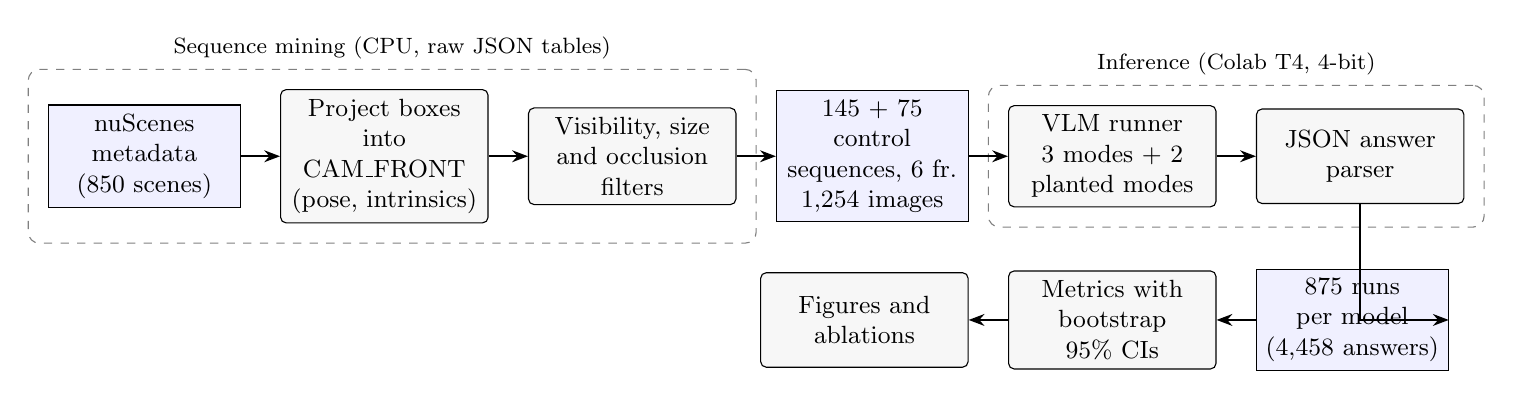
\begin{tikzpicture}[
  font=\small, node distance=4mm and 5mm,
  box/.style={draw, rounded corners=2pt, align=center, minimum height=12mm, text width=24mm, fill=gray!6},
  data/.style={draw, align=center, minimum height=12mm, text width=22mm, fill=blue!6},
  arr/.style={-{Stealth[length=2mm]}, thick}]
  \node[data] (meta) {nuScenes\\metadata\\(850 scenes)};
  \node[box, right=of meta] (proj) {Project boxes\\into CAM\_FRONT\\(pose, intrinsics)};
  \node[box, right=of proj] (filt) {Visibility, size\\and occlusion\\filters};
  \node[data, right=of filt] (seq) {145 + 75 control\\sequences, $6$ fr.\\1{,}254 images};
  \node[box, right=of seq] (run) {VLM runner\\3 modes + 2\\planted modes};
  \node[box, right=of run] (parse) {JSON answer\\parser};
  \node[box, below=8mm of run] (metric) {Metrics with\\bootstrap 95\% CIs};
  \node[box, left=of metric] (fig) {Figures and\\ablations};
  \node[data, right=of metric] (res) {875 runs\\per model\\(4{,}458 answers)};
  \draw[arr] (meta) -- (proj);
  \draw[arr] (proj) -- (filt);
  \draw[arr] (filt) -- (seq);
  \draw[arr] (seq) -- (run);
  \draw[arr] (run) -- (parse);
  \draw[arr] (parse) |- (res);
  \draw[arr] (res) -- (metric);
  \draw[arr] (metric) -- (fig);
  \begin{scope}[on background layer]
    \node[draw=gray, dashed, rounded corners, fit=(meta)(proj)(filt), inner sep=2.5mm, label={[font=\footnotesize]above:Sequence mining (CPU, raw JSON tables)}] {};
    \node[draw=gray, dashed, rounded corners, fit=(run)(parse), inner sep=2.5mm, label={[font=\footnotesize]above:Inference (Colab T4, 4-bit)}] {};
  \end{scope}
\end{tikzpicture}
\caption{Pipeline. Positive and control sequences are mined on a CPU from the nuScenes metadata alone; only the 1{,}254 images they use are extracted. Positive sequences are run in five modes and control sequences in two, answers are parsed from JSON, and metrics are computed with scene-level bootstrap confidence intervals.}
\label{fig:pipeline}
\end{figure*}

Fig.~\ref{fig:pipeline} shows the pipeline. It reads the raw nuScenes JSON tables directly, without the nuScenes development kit, and keeps only front-camera keyframes and pedestrian annotations in memory so that the full trainval metadata loads in about 40\,s.

\subsection{Sequence mining}

For each pedestrian annotation with global position $\mathbf{p}_g$ we compute its position in the front camera frame,
\begin{equation}
\mathbf{p}_c = R_c^{\top}\!\left(R_e^{\top}(\mathbf{p}_g - \mathbf{t}_e) - \mathbf{t}_c\right),
\end{equation}
where $(R_e, \mathbf{t}_e)$ is the ego pose of that camera image and $(R_c, \mathbf{t}_c)$ the camera extrinsics. The pedestrian is in view if $z_c > 0.5$\,m and its projected centre $K\mathbf{p}_c / z_c$ falls inside the $1600\times900$ image, with $K$ the intrinsic matrix. Its on-screen height is approximated as $h_{\text{px}} \approx f_x h / z_c$, with $h$ the box height and $f_x$ the focal length.

A sequence is $T=6$ consecutive keyframes (3\,s at 2\,Hz) in which one pedestrian stays in view, and it must satisfy:
\begin{enumerate}
  \item the first frame has nuScenes visibility level 1 (0--40\% visible);
  \item the \emph{evidence frame} $k$ is the first with level 4 (80--100\%), with $h_{\text{px}} \ge 40$ at frame $k$;
  \item every frame before $k$ has level $\le 2$, and no other pedestrian is clearly visible (level $\ge 3$) before $k$;
  \item $k \le T-2$, so that at least one frame follows the evidence.
\end{enumerate}
Condition~3 removes sequences in which the question can be answered from a different pedestrian. One sequence is kept per pedestrian. Sequences of different pedestrians in the same scene can share frames: 59 of the 804 images appear in more than one sequence. On nuScenes v1.0-trainval this yields 145 sequences from 120 scenes with $k \in \{1,\dots,4\}$; the mini split yields only 2.

\subsection{Control sequences}

A control sequence is $T=6$ consecutive keyframes in which no pedestrian, bicycle or motorcycle can be seen at all. Cyclists are excluded because nuScenes labels them as the vehicle, not as a person, while a VLM may call them pedestrians. The centre test above would miss a box whose centre is outside the image but whose edge is inside it, so controls use a stricter test: all eight corners of every such box are projected, and a frame is rejected if any projected corner reaches the image or the box straddles the camera plane ($z_c \le 0.1$\,m for some corners). Pedestrian-free windows are easier to find at night and in rain, so unconstrained controls had about twice the positives' share of both. We therefore match the controls to the positive sequences on conditions, labelling each scene night, rain or clear from its nuScenes description and selecting controls in the same proportions. Within each condition we take one window per scene, preferring scenes that also contain positive sequences, and copy $k$ from a positive sequence of the same scene (or a random one), so planted modes see the same mix of planted turns. This yields 75 control sequences (450 images) from 75 scenes, 52 of which also contain positive sequences, with 61 clear, 9 rain and 5 night scenes; ground truth is ``no'' on every frame. Missing annotations do not prove an empty frame, since distant pedestrians can be unlabelled; we inspected the control images by eye and saw no pedestrians. They span daylight and rain, including frames partly blurred by water on the lens.

\subsection{Query and modes}

At every frame the model receives the image and the prompt ``You are the perception module of an autonomous vehicle. The image is from the front camera. Is there a pedestrian in the most recent image?'' and must answer in JSON with \emph{present} (yes/no), \emph{confidence}, \emph{evidence} and a driving \emph{action} (proceed, slow or stop). Let $q$ be this prompt, $I_t$ the image at frame $t$ and $a_t$ the answer. The three modes are
\begin{align}
\text{stateless:}\quad & a_t = f(I_t, q),\\
\text{stateful:}\quad & a_t = f\big((I_0,q,a_0),\dots,(I_{t-1},q,a_{t-1}), I_t, q\big),\\
\text{reconsider:}\quad & \text{stateful with } q \leftarrow r \oplus q \text{ for } t>0,
\end{align}
where $r$ is ``This is a new frame. Your earlier answers may have been wrong; judge only from this image.'' Stateless inference is equivalent to resetting the history at every frame. At $t=0$ all three modes receive the same input.

\textbf{Planted beliefs.} In the stateful modes the wrong belief at $k-1$ is the model's own, and often a fair call on an occluded frame. The two planted modes instead write a fixed answer $\hat a$ into the history for every frame before the evidence frame, without querying the model:
\begin{equation}
a_t = \begin{cases} \hat a, & t < k,\\ f(H_t, I_t, q), & t \ge k, \end{cases}
\end{equation}
where $H_t = (I_0,q,\hat a),\dots,(I_{k-1},q,\hat a),(I_k,q,a_k),\dots,(I_{t-1},q,a_{t-1})$. For \emph{planted-no}, $\hat a$ is a JSON answer with present ``no'', confidence 0.9, evidence ``no pedestrian is visible'' and action ``proceed''; for \emph{planted-yes} it is the corresponding ``yes'' answer with evidence ``a pedestrian is visible'' and action ``slow''. The images are the same as in the stateful mode; only the answers differ, so comparing planted-no with planted-yes isolates the effect of the answer text. Evidence grows along two axes: the number of planted turns ($k=1$ to 4) and the frames after $k$, in which the pedestrian stays at least 80\% visible and usually grows. On control sequences we run stateless and planted-yes, where the planted ``yes'' is the wrong belief.

\subsection{Metrics}

Ground truth is ``present'' on every frame of a positive sequence and ``absent'' on every frame of a control sequence. Let $c^m_{s,t}\in\{0,1\}$ indicate a correct answer in mode $m$ for sequence $s$ at frame $t$. Planted frames are not model output and are left out of every per-frame metric.

\textbf{Visible-without-history accuracy} is our headline metric. With $V=\{s : c^{\text{SL}}_{s,k_s}=1\}$ the sequences whose evidence frame the model detects statelessly,
\begin{equation}
\text{VWH}^m = \frac{1}{|V|}\sum_{s\in V} c^m_{s,k_s}.
\end{equation}
Because every frame in $V$ is perceivable by the same model without history, $1-\text{VWH}^m$ is the share of detections removed by the history. On control sequences the same definition, with $V$ the evidence frames the model correctly calls empty without history, gives \emph{empty-without-history accuracy}. An exact McNemar test on the evidence frame counts both directions: history turning a correct stateless answer wrong, and the reverse.

\textbf{Post-evidence accuracy} $\text{PEA}^m_s$ is the mean of $c^m_{s,t}$ over $t \ge k_s$; we report the paired difference $\Delta = \frac{1}{N}\sum_s (\text{PEA}^{\text{SF}}_s - \text{PEA}^{\text{SL}}_s)$.
\textbf{Persistence rate} is the share of sequences wrong at $k-1$ that are still wrong at $k+1$, after two contradictory frames. At $k-1$ the pedestrian is at most 40\% visible in 121 of 145 sequences, so a ``no'' there is often a reasonable perceptual call; we call it an \emph{initial miss}, not a hallucination. The hallucination we measure is a ``no'' on the evidence frame that the same model answers correctly without history, which is what VWH counts. Which sequences have an initial miss depends on the mode, so when comparing modes we report persistence on the sequences that both modes miss at $k-1$.
\textbf{Correction latency} is the number of frames from $k$ to the first correct answer.
\textbf{Copy rate} is the share of answers at $t\ge1$ identical, character for character, to the answer at $t-1$.
\textbf{False-positive rate} is the share of control-sequence answers reporting a pedestrian.
\textbf{Safety-action accuracy} compares the predicted action with a rule-based label (stop within 15\,m and 2.5\,m of the camera axis, slow within 15\,m, otherwise proceed).
All intervals are 95\% percentile bootstrap intervals with 1{,}000 resamples~\cite{efron1979bootstrap}. Sequences from the same scene share conditions and sometimes frames, so the bootstrap resamples scenes rather than sequences.

\begin{figure*}[!t]
\centering
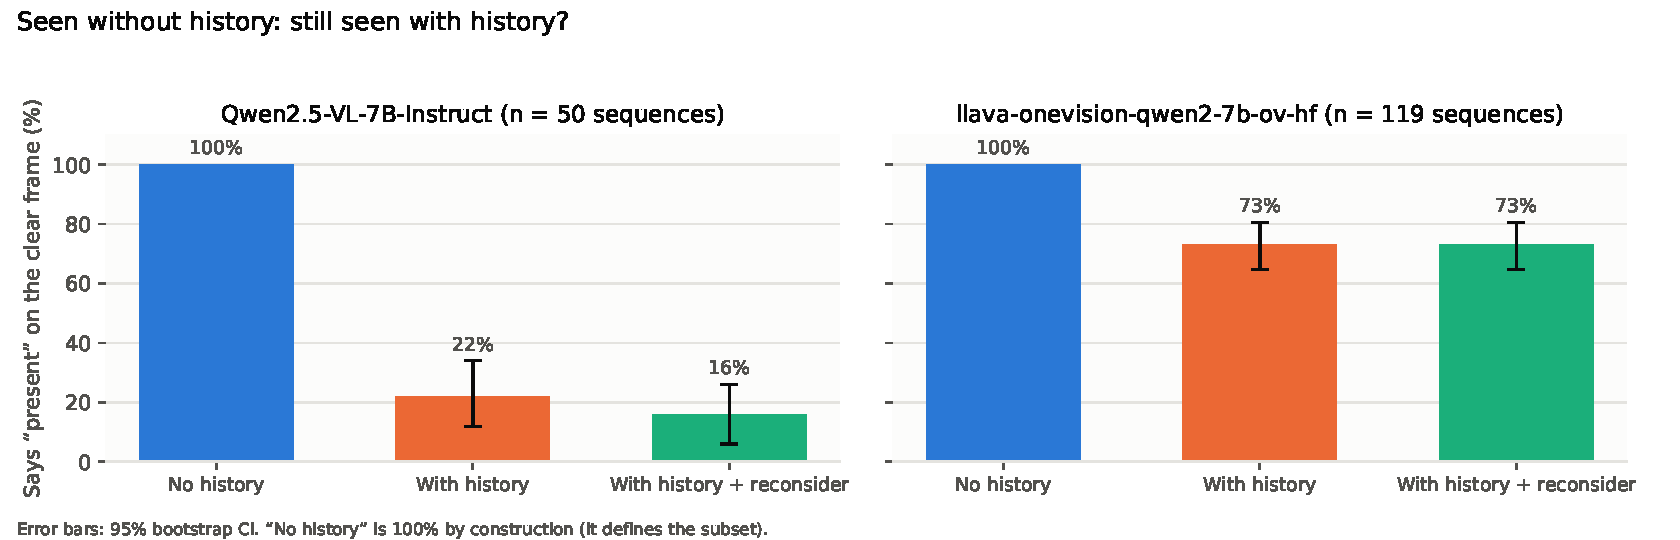
\includegraphics[width=\textwidth]{visible_without_history.pdf}
\caption{Visible-without-history accuracy. Among evidence frames each model answers correctly without history (Qwen $n=43$, LLaVA $n=107$), the share it still answers correctly with its own history, with a reconsider instruction, and after planted ``no'' or ``yes'' answers (hatched). Error bars: 95\% scene-level bootstrap CIs.}
\label{fig:vwh}
\end{figure*}

\begin{figure*}[!t]
\centering
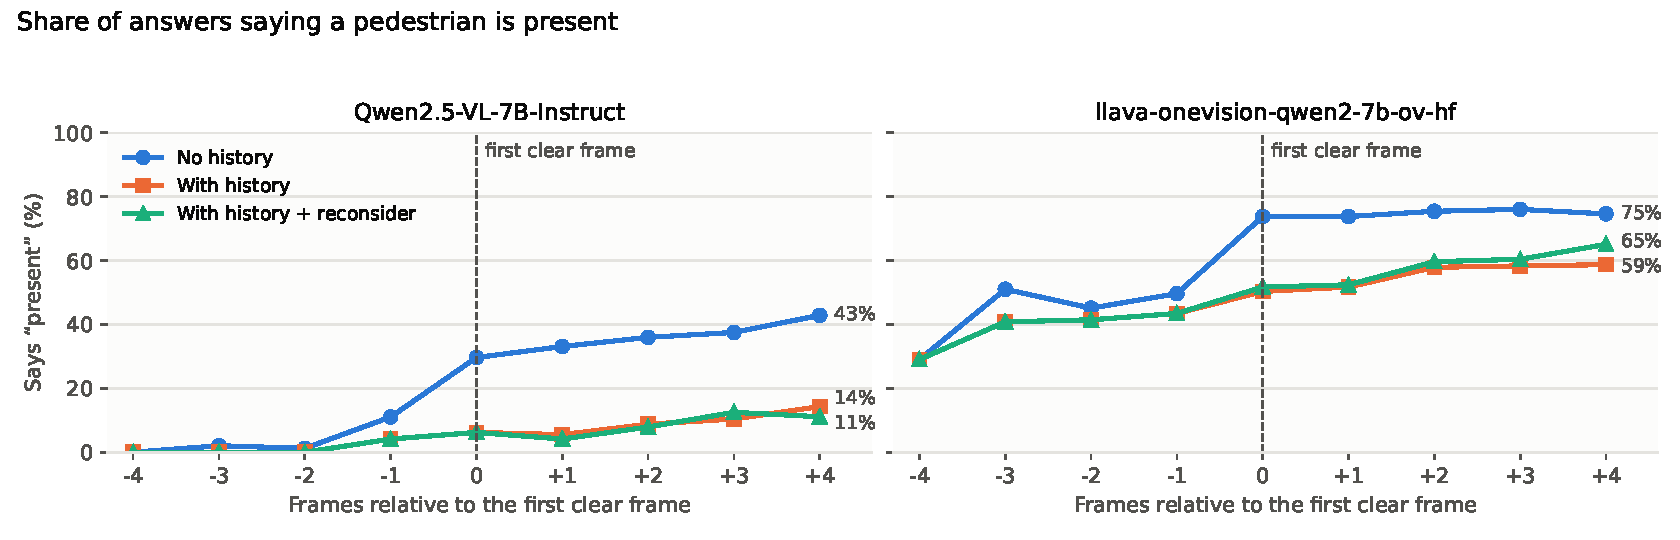
\includegraphics[width=\textwidth]{yes_by_frame.pdf}
\caption{Share of answers reporting a pedestrian, by frame relative to the evidence frame (offsets reached by at least 20 sequences). Without history, both models respond to the evidence frame; with history, the response largely disappears.}
\label{fig:frames}
\end{figure*}

% ---------------------------------------------------------------------------
\section{Experiments and Ablation Studies}

\subsection{Setup}

Both models run on a Google Colab NVIDIA T4 (16\,GB) with Hugging Face Transformers, 4-bit bitsandbytes weights and fp16 compute, greedy decoding and at most 128 new tokens. Qwen2.5-VL-7B-Instruct receives images resized to a longest side of 1024\,px. LLaVA-OneVision-Qwen2-7B tiles each image, so a six-frame history at 1024\,px needs 27.7k prompt tokens and exhausts the T4 (Table~\ref{tab:profile}); it therefore runs at 768\,px. Each model answers 145 sequences $\times$ 3 modes $\times$ 6 frames $=2{,}610$ queries in the unplanted modes, $2\times563$ in the planted modes (planted frames need no query) and $450+272=722$ on control sequences. Package versions are pinned (Transformers 5.24.1, Accelerate 1.16.0, bitsandbytes 0.50.2) and every result records its settings and versions. The stateless mode is the baseline, equivalent to resetting the history.

\subsection{Main results}

\begin{table}[t]
\centering
\caption{Main results (145 sequences per model; 95\% scene-level bootstrap CIs). Persistence is conditioned on an initial miss at $k{-}1$ in that mode, so its denominator differs by mode.}
\label{tab:main}
\setlength{\tabcolsep}{3pt}
\begin{tabular}{@{}llccc@{}}
\toprule
Model & Metric & Stateless & Stateful & Reconsider\\
\midrule
\multirow{4}{*}{Qwen}  & Post-evid. acc. (\%) & 33 [26,40] & 8 [4,12] & 7 [4,11]\\
                       & Persistence (\%)     & 74 [66,81] & 96 [92,99] & 97 [94,100]\\
                       & Initial miss ($n$)   & 129 & 139 & 139\\
                       & Never corrected ($n$) & 67 & 123 & 124\\
\midrule
\multirow{4}{*}{LLaVA} & Post-evid. acc. (\%) & 74 [67,80] & 52 [43,61] & 54 [46,62]\\
                       & Persistence (\%)     & 40 [27,52] & 85 [77,93] & 84 [76,92]\\
                       & Initial miss ($n$)   & 73 & 82 & 82\\
                       & Never corrected ($n$) & 13 & 68 & 62\\
\bottomrule
\end{tabular}
\end{table}

Table~\ref{tab:main} gives the main results. The paired stateful-minus-stateless difference in post-evidence accuracy is $-25$ points [$-32$, $-19$] for Qwen and $-22$ points [$-30$, $-14$] for LLaVA; both exceed the 10-point threshold we set in advance for a meaningful effect. On the sequences that both modes miss at $k-1$ (Qwen $n=129$, LLaVA $n=68$), history raises persistence from 74\% to 97\% for Qwen and from 41\% to 84\% for LLaVA.

The models differ sharply in perception, so post-evidence accuracy alone mixes two effects. Fig.~\ref{fig:vwh} removes perception: on evidence frames that the model detects without history, Qwen with history still detects the pedestrian in 21\% [9, 36] of sequences and LLaVA in 60\% [50, 69]. History therefore removes most of Qwen's correct detections and 40\% of LLaVA's. The effect is not one-sided by construction: on the evidence frame, history turns a correct stateless answer into a miss in 34 sequences for Qwen and 43 for LLaVA, and does the reverse in 0 and 9 (exact McNemar test, $p<10^{-9}$ and $p<10^{-5}$).

Fig.~\ref{fig:frames} shows the same effect frame by frame. Without history, the share of ``present'' answers rises at the evidence frame, from 11\% to 30\% for Qwen and from 50\% to 74\% for LLaVA. With history it rises only from 4\% to 6\% for Qwen and from 43\% to 50\% for LLaVA.

\begin{figure*}[!t]
\centering
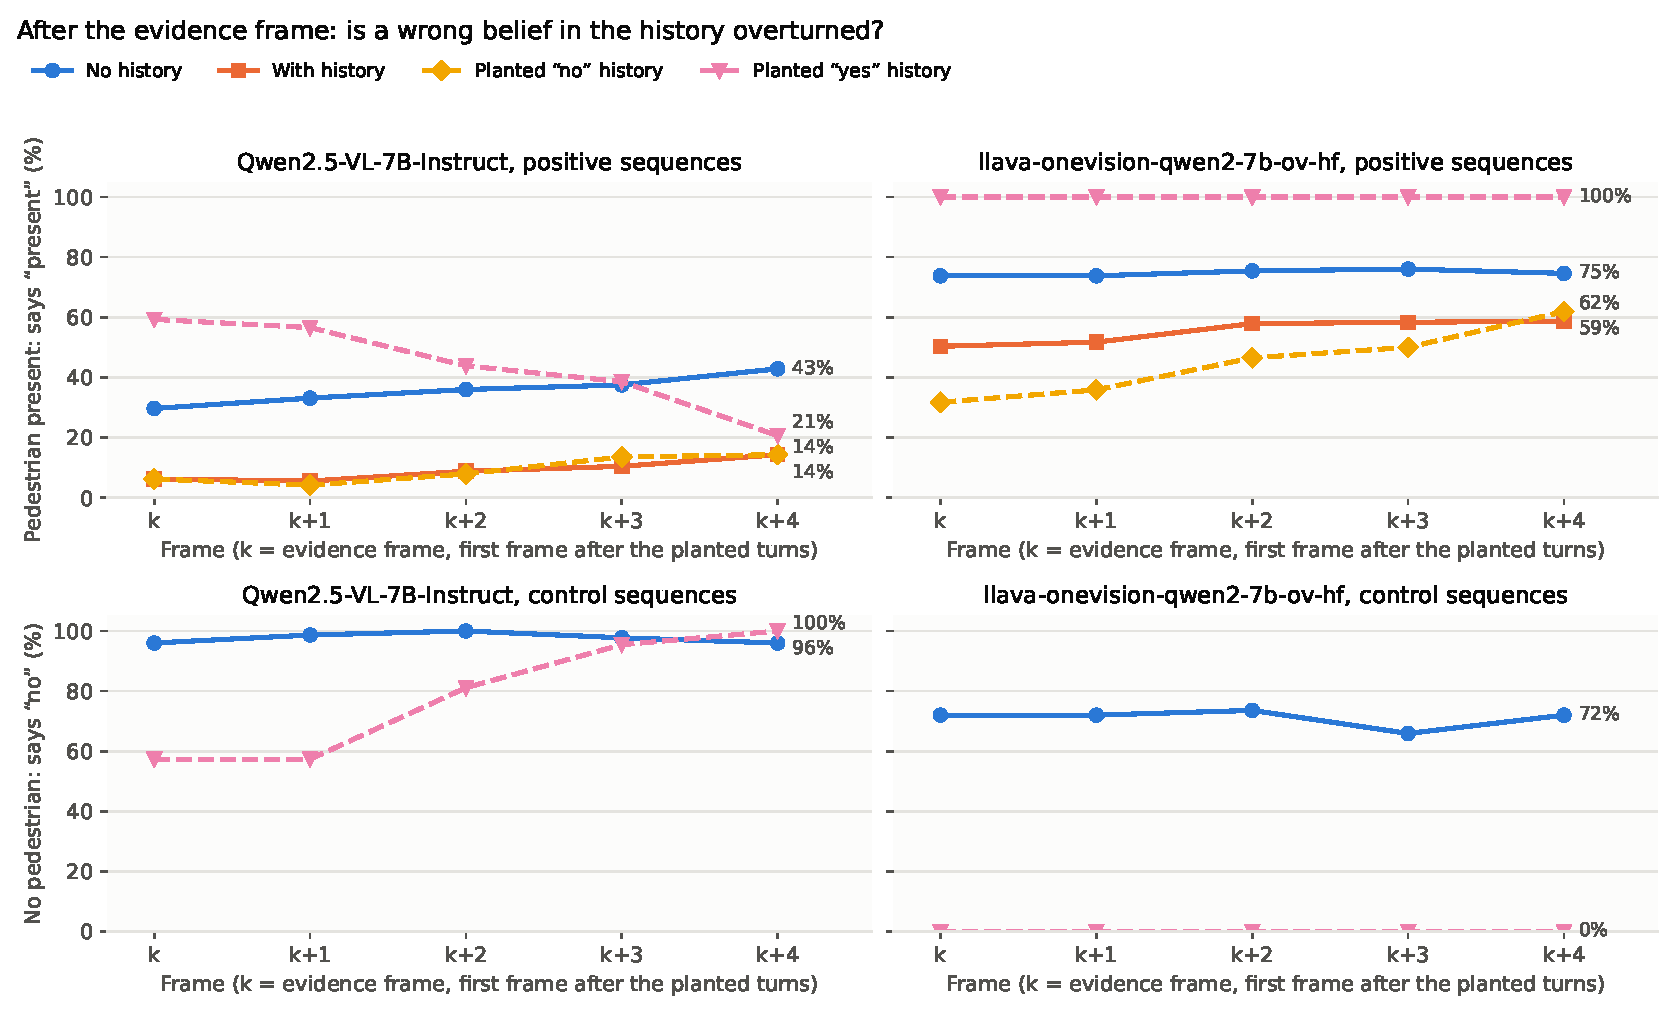
\includegraphics[width=\textwidth]{planted_belief.pdf}
\caption{Accuracy from the evidence frame $k$ on (offsets reached by at least 20 sequences). Later offsets are reached only by sequences with a small $k$, i.e.\ few planted turns, so the curves mix time since the evidence with the number of planted turns. Top: positive sequences, with no history, the model's own history, and a planted ``no'' or ``yes'' before $k$. Bottom: control sequences, where the planted ``yes'' is the wrong belief.}
\label{fig:planted}
\end{figure*}

\subsection{Mechanism: answer copying}

\begin{table}[t]
\centering
\caption{Answer copying across frames ($t\ge1$, 725 per mode).}
\label{tab:copy}
\begin{tabular}{@{}lcccc@{}}
\toprule
& \multicolumn{2}{c}{Qwen} & \multicolumn{2}{c}{LLaVA}\\
\cmidrule(lr){2-3}\cmidrule(lr){4-5}
& Stateless & Stateful & Stateless & Stateful\\
\midrule
Identical to previous answer (\%) & 30 & 78 & 36 & 93\\
Same yes/no as previous answer (\%) & 84 & 97 & 77 & 98\\
``no''$\to$``yes'' switches ($n$) & 82 & 17 & 106 & 15\\
\bottomrule
\end{tabular}
\end{table}

With history, both models mostly repeat their previous answer character for character, including the evidence sentence (Table~\ref{tab:copy}). Without history the same models switch from ``no'' to ``yes'' 82 and 106 times across the 145 sequences; with history only 17 and 15 times. With history, 97\% and 98\% of answers keep the previous yes/no decision.

\subsection{Planted beliefs}

\begin{table}[t]
\centering
\caption{Planted beliefs (95\% scene-level bootstrap CIs). VWH and EWH: evidence-frame accuracy on the frames the model answers correctly without history (Qwen $n=43$ and 72, LLaVA $n=107$ and 54). Never corrected: sequences with no correct answer from $k$ on.}
\label{tab:planted}
\setlength{\tabcolsep}{3pt}
\begin{tabular}{@{}llcc@{}}
\toprule
& Metric & Qwen & LLaVA\\
\midrule
\multirow{4}{*}{\shortstack[l]{Positive,\\planted ``no''}} & VWH (\%) & 21 [8,36] & 43 [32,53]\\
                            & Post-evid. acc. (\%) & 7 [4,12] & 37 [29,46]\\
                            & Persistence (\%) & 96 [92,99] & 64 [55,73]\\
                            & Never corrected ($n$/145) & 127 & 83\\
\midrule
\multirow{2}{*}{\shortstack[l]{Positive,\\planted ``yes''}} & VWH (\%) & 91 [81,98] & 100\\
                            & Post-evid. acc. (\%) & 58 [49,65] & 100\\
\midrule
\multirow{2}{*}{\shortstack[l]{Control,\\no history}} & Says ``present'' (\% of 450) & 1.6 & 31\\
                            & Post-evid. acc. (\%) & 98 [96,100] & 70 [63,77]\\
\midrule
\multirow{4}{*}{\shortstack[l]{Control,\\planted ``yes''}} & EWH (\%) & 57 [46,68] & 0\\
                            & Post-evid. acc. (\%) & 58 [47,69] & 0\\
                            & Persistence (\%) & 43 [31,53] & 100\\
                            & Never corrected ($n$/75) & 31 & 75\\
\bottomrule
\end{tabular}
\end{table}

The planted modes test the effect causally (Table~\ref{tab:planted}, Fig.~\ref{fig:planted}). With a planted ``no'', Qwen still detects 21\% [8, 36] of the evidence frames it detects without history, the same as with its own history, and never corrects 127 of the 145 sequences. LLaVA still detects 43\% [32, 53], fewer than the 60\% with its own history, because its own history at $k-1$ is often a ``yes''. With a planted ``yes'' on the same images, the detections return (91\% and 100\%), so the answer text, not the images, drives the error. LLaVA overturns the planted ``no'' only slowly: in sequences with one planted turn, its accuracy rises from 48\% at $k$ to 62\% at $k+4$. More planted turns make the belief stronger: LLaVA detects 67\% of perceivable pedestrians after one planted ``no'' and 14\% after four ($n=45$ and 21). Qwen shows no such trend; one planted ``no'' is already enough (26\%, $n=19$).

On control sequences without history, Qwen reports a pedestrian on 1.6\% of frames, LLaVA on 31\% (in 52 of the 75 sequences). After a planted ``yes'', LLaVA answers ``yes'' on every remaining frame of all 75 sequences, copying the planted answer verbatim, so its empty-without-history accuracy is 0\% ($n=54$). Qwen calls 57\% [46, 68] of the empty frames it gets right without history empty again, but this depends on the number of planted turns: 100\% after one ($n=23$), 89\% after two ($n=18$), 11\% after three ($n=9$) and 5\% after four ($n=22$). Within each group the answers barely change over the following frames; the rise of the Qwen control curve in Fig.~\ref{fig:planted} comes from only one-turn sequences reaching $k+4$. Qwen thus resists a single planted ``yes'' but not a single planted ``no'', while repeated wrong answers in either direction override what it sees.

\begin{figure*}[!t]
\centering
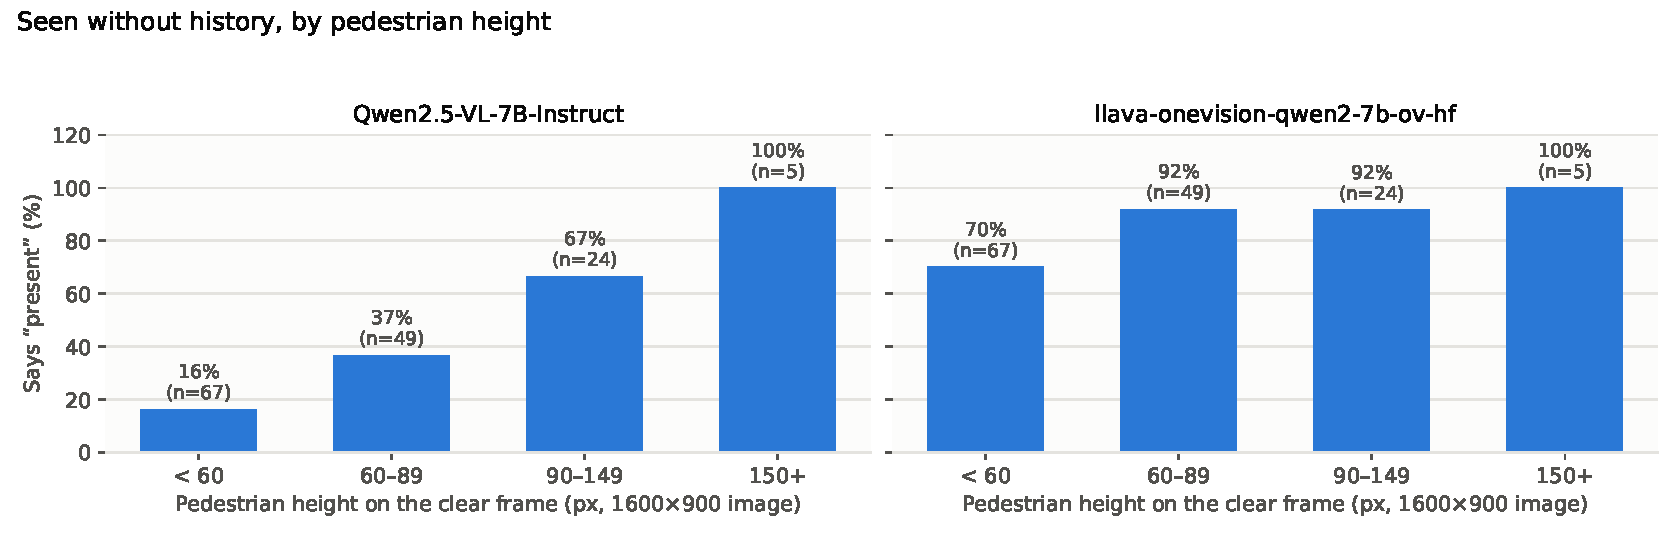
\includegraphics[width=\textwidth]{seen_by_size.pdf}
\caption{Stateless detection on the evidence frame by pedestrian height at full resolution. Qwen misses most pedestrians under 90\,px, which is why the visible-without-history subset is needed.}
\label{fig:size}
\end{figure*}

\subsection{Ablations}

\begin{table}[t]
\centering
\caption{Ablations on the visible-without-history subset: stateful accuracy (\%) on the evidence frame unless noted. $n$ in parentheses.}
\label{tab:ablation}
\setlength{\tabcolsep}{4pt}
\begin{tabular}{@{}llcc@{}}
\toprule
Factor & Level & Qwen & LLaVA\\
\midrule
\multirow{2}{*}{Stateful answer at $k{-}1$} & ``yes'' & 60 (5) & 100 (54)\\
                                            & ``no''  & 16 (38) & 19 (53)\\
\midrule
\multirow{4}{*}{\shortstack[l]{Evidence index $k$\\(earlier turns)}} & 1 & 16 (19) & 64 (45)\\
                                         & 2 & 25 (12) & 58 (26)\\
                                         & 3 & 0 (6)   & 67 (15)\\
                                         & 4 & 50 (6)  & 48 (21)\\
\midrule
\multirow{4}{*}{\shortstack[l]{Planted ``no'' turns $k$\\(planted-no accuracy)}} & 1 & 26 (19) & 67 (45)\\
                                         & 2 & 17 (12) & 35 (26)\\
                                         & 3 & 0 (6)   & 27 (15)\\
                                         & 4 & 33 (6)  & 14 (21)\\
\midrule
\multirow{3}{*}{\shortstack[l]{Pedestrian height\\at $k$ (px)}} & $<60$  & 0 (8)  & 46 (39)\\
                                            & 60--89 & 0 (14)  & 62 (42)\\
                                            & $\ge 90$ & 43 (21) & 77 (26)\\
\bottomrule
\end{tabular}
\end{table}

Table~\ref{tab:ablation} varies one factor at a time on the visible-without-history subset.

\textbf{Previous answer.} The stateful answer on the clearly visible frame is almost fully determined by the answer one frame earlier. After a ``yes'' LLaVA stays correct in all 54 sequences and Qwen in 3 of 5; after a ``no'', only 16\% (Qwen) and 19\% (LLaVA) of pedestrians that the same model sees without history are reported. Because these answers are the model's own, the planted-belief experiment above tests the same dependence with a belief the model did not form.

\textbf{History length.} With the model's own history, the number of earlier turns before the evidence frame ($k=1$ to 4) shows no consistent trend for either model, so a single wrong turn is enough to anchor the answer. With a planted ``no'', LLaVA's accuracy falls steadily with the number of planted turns, from 67\% to 14\%; Qwen's shows no trend.

\textbf{Pedestrian size.} Larger pedestrians partly overcome the history: stateful accuracy rises to 43\% (Qwen) and 77\% (LLaVA) for pedestrians at least 90\,px tall. Size also governs stateless perception: without history Qwen detects 12\% of evidence-frame pedestrians under 60\,px and all 5 above 150\,px, while LLaVA detects 58\% and 100\% (Fig.~\ref{fig:size}).

\textbf{Mining thresholds.} Table~\ref{tab:mining} shows how the sequence count depends on the sequence length and minimum pedestrian height. We chose 6 frames and 40\,px: it is the only setting above 100 sequences that keeps four frames after the earliest evidence frame, which the latency metric needs.

\begin{table}[t]
\centering
\caption{Sequences mined from nuScenes v1.0-trainval.}
\label{tab:mining}
\begin{tabular}{@{}lccc@{}}
\toprule
& \multicolumn{3}{c}{Minimum height at evidence frame}\\
\cmidrule(lr){2-4}
Frames per sequence & 40\,px & 60\,px & 80\,px\\
\midrule
4 & 177 & 104 & 52\\
5 & 163 & 91 & 47\\
6 & \textbf{145} & 81 & 40\\
\bottomrule
\end{tabular}
\end{table}

\textbf{Mitigation.} The reconsider instruction gives 7\% (Qwen) and 54\% (LLaVA) post-evidence accuracy, no better than plain history (8\% and 52\%, Table~\ref{tab:main}), and 21\% [8, 36] and 62\% [51, 71] visible-without-history accuracy. It lowers Qwen's verbatim copy rate from 78\% to 57\%, but Qwen still keeps the previous yes/no decision in 96\% of answers: it rewords the answer without revising it. LLaVA's copy rate is unchanged (92\%). Resetting the history (stateless) restores accuracy to 33\% and 74\%.

\begin{figure*}[!t]
\centering
\includegraphics[width=\textwidth]{{examples_Qwen2.5-VL-7B-Instruct}.pdf}\\[2mm]
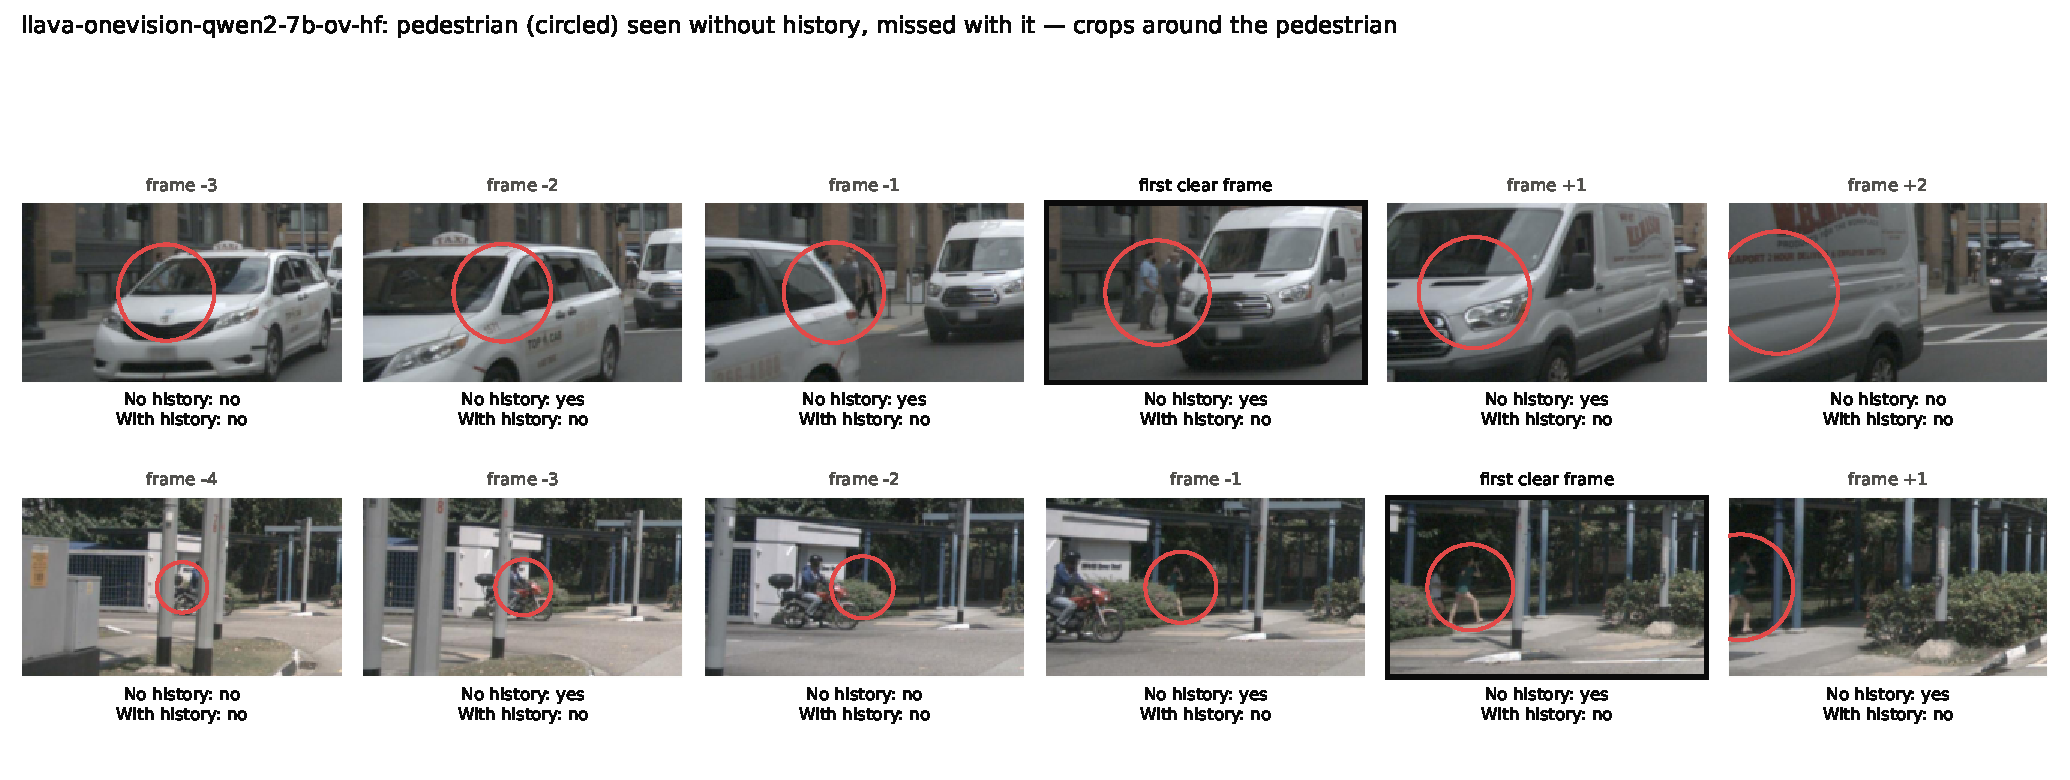
\includegraphics[width=\textwidth]{examples_llava-onevision-qwen2-7b-ov-hf.pdf}
\caption{Example sequences, cropped around the annotated pedestrian (circled); the evidence frame has a black border. Top: Qwen2.5-VL. Bottom: LLaVA-OneVision. In each, the model detects the pedestrian without history but keeps answering ``no'' with history.}
\label{fig:examples}
\end{figure*}

\subsection{Latency and memory}

\begin{table}[t]
\centering
\caption{Prompt length per query, measured with each model's own processor on a real sequence, for a single frame (stateless) and the last frame of a six-frame history (stateful).}
\label{tab:profile}
\setlength{\tabcolsep}{4pt}
\begin{tabular}{@{}lcccc@{}}
\toprule
& \multicolumn{2}{c}{Prompt tokens} & & \\
\cmidrule(lr){2-3}
Model, image size & 1 frame & 6-frame hist. & Ratio & Fits T4?\\
\midrule
Qwen, 1024\,px  & 875     & 5{,}345  & 6.1$\times$ & Yes\\
Qwen, 768\,px   & 503     & 3{,}113  & 6.2$\times$ & Yes\\
LLaVA, 1024\,px & 4{,}586 & 27{,}661 & 6.0$\times$ & No (OOM)\\
LLaVA, 768\,px  & 2{,}464 & 14{,}929 & 6.1$\times$ & Yes\\
\bottomrule
\end{tabular}
\end{table}

Stateful inference grows the prompt linearly with the number of frames: the last query of a six-frame history is about six times longer than a stateless query (Table~\ref{tab:profile}). LLaVA's tiling makes each frame 2.8$\times$ as long as Qwen's even at a smaller image size. At 1024\,px its six-frame prompt reaches 27{,}661 tokens, and the run failed with 13.7\,GiB in use on the 14.6\,GiB device; 768\,px halves the prompt and fits. Since attention cost grows with prompt length, keeping the history is not only less accurate than resetting it but also more expensive per query. Measured per query on the T4, the median latency is 3.7\,s (Qwen) and 4.2\,s (LLaVA) without history and 7.2\,s and 10.8\,s with it, rising to 10.7\,s and 21.9\,s at the sixth frame. Peak GPU memory reaches 7.0\,GB and 8.8\,GB.

\subsection{Qualitative results}

Fig.~\ref{fig:examples} shows two sequences per model. In the first LLaVA example, the model without history detects the pedestrian on four consecutive frames, while the model with history answers ``no'' on all six.

% ---------------------------------------------------------------------------
\section{Failure Analysis, Negative Results and Limitations}

\textbf{Anchoring on the model's own answer.} The dominant failure is that a stateful model treats its previous answer as evidence. After a ``no'' at $k-1$, 84\% (Qwen) and 81\% (LLaVA) of perceivable pedestrians are missed on the clearly visible frame. The root cause is visible in the outputs: the answer, including its free-text evidence (``There are no pedestrians visible in the image.''), is copied verbatim.

\textbf{Negative result: prompting does not fix it.} Telling the model that its earlier answers may be wrong does not change accuracy, nor how often the previous yes/no decision is kept (96--97\%); Qwen only rewords its answers more often. The bias is not removed by an instruction placed in the same context that contains the anchoring answers; only removing those answers helps.

\textbf{Persistence or copying?} Inertia runs both ways: with history, LLaVA never switches from ``yes'' to ``no'' (64 times without history), and Qwen does so 8 times (35 without). On positive sequences only the harmful direction counts as an error, so these runs alone cannot tell a held belief that the pedestrian is absent from repeating the last answer. The control sequences separate the two. A planted wrong ``yes'' on empty frames removes all of LLaVA's correct ``no'' answers, more than a planted ``no'' removes of its detections (57\%). For Qwen it removes 43\% overall and 95\% after four planted turns, against 79\% for a planted ``no''. Wrong answers persist in both directions, so the failure is answer copying, not a belief specific to absence. The one asymmetry is that Qwen ignores a single planted ``yes'' but not a single planted ``no''.

\textbf{Overconfidence.} Qwen reports a mean confidence of 0.90--0.93 on wrong answers and 0.80--0.88 on correct ones in every mode, so its confidence cannot flag persistent errors. LLaVA reports a confidence near 0 for every ``no'' answer, treating the field as a probability of presence, so its confidences are not comparable.

\textbf{Perception failures.} Qwen at 1024\,px detects only 12\% of pedestrians under 60\,px on the evidence frame, even without history. We handle this with the visible-without-history subset instead of reporting raw accuracy. LLaVA errs the other way: without history it reports a pedestrian on 31\% of empty control frames, so some of its detections on positive sequences, and of the visible-without-history subset, are likely ``yes'' answers that happen to be right.

\textbf{Format failures.} LLaVA answered with a bare ``Yes'' or ``No'' instead of JSON on 750 of 2{,}610 frames in the three unplanted modes (186 without history, 282 in each mode with history). The yes/no answer is still recovered, but no action is given; these frames count as unsafe, which inflates LLaVA's unsafe-action rate (26\% stateless, 37\% stateful).

\textbf{Format copying.} The bare replies are how LLaVA says ``no''. Without history, none of its 563 ``yes'' answers is bare, but 186 of its 307 ``no'' answers are (61\%), as are 222 of the 450 answers on control frames. With history, the format of the first answer is copied for the rest of the sequence. A bare reply was followed by another bare reply 235 times out of 235, and a JSON reply was never followed by a bare one (0 of 490). The 282 bare frames per stateful mode are therefore 47 sequences that start with a bare ``No'', six frames each; nine of these frames are a bare ``Yes'' that keeps the format but not the answer. The planted modes, whose history starts with our JSON answers, produce no bare replies. The format also changes how strongly the history anchors the answer. On evidence frames LLaVA detects without history, it still detects 6\% ($n=31$) with history in the sequences that start bare, against 82\% ($n=76$) in those that start with JSON. After a ``no'' at $k-1$ the split is 6\% ($n=31$) against 36\% ($n=22$). The bare-start sequences are somewhat harder, with 62\% post-evidence accuracy without history against 80\%, but not by enough to explain this gap. LLaVA's history effect is therefore concentrated in sequences where it copies a terse ``No'', and it depends on how often LLaVA chooses that format. That choice is sensitive to the question wording: in an earlier run that asked about ``the image'' rather than ``the most recent image'', 7 rather than 47 sequences started with a bare reply, and 10\% rather than 61\% of stateless ``no'' answers were bare.

\textbf{Label failures.} nuScenes visibility is aggregated over all six cameras, so a frame labelled 80--100\% visible can be occluded in the front camera. We found such a case by inspection (a pedestrian behind a passing van); the visibility labels were not reviewed manually. The visible-without-history metric is robust to this because it only counts frames the model itself detects.

\textbf{Limitations.} (i) The 75 control sequences are run only without history and with a planted ``yes'', and missing annotations do not guarantee an empty frame. (ii) Action labels are rule-based and 95\% are ``proceed'', so safety-action accuracy (Qwen 46--51\%, LLaVA 22--30\% balanced) is weak evidence; the rule considers only pedestrians, including occluded ones, and ignores vehicles. (iii) The two models use different image sizes to fit the GPU, so absolute accuracies are not directly comparable; each model's history effect is. (iv) Only object presence is tested, not attributes or spatial relations. (v) Two 7B models were evaluated, both with 4-bit weights, including the vision encoder, which may reduce small-object detection. (vi) The planted answers use one fixed wording, which differs from each model's own style (LLaVA, for example, sometimes answers with a bare ``No''), so a planted history is not identical in form to a natural one. (vii) LLaVA's history effect depends on its output format, which depends on the question wording, so its size is specific to our prompt.

% ---------------------------------------------------------------------------
\section{Conclusion and Future Work}

Keeping a conversation history makes vision-language models repeat their earlier ``no pedestrian'' answers after the pedestrian becomes clearly visible. Across 145 nuScenes sequences, history removes 79\% of Qwen2.5-VL's and 40\% of LLaVA-OneVision's otherwise correct detections on the clearest frame, and the mechanism is answer copying. A planted wrong ``no'' removes 79\% and 57\% of them, and a planted wrong ``yes'' on empty frames is kept by LLaVA on every frame and by Qwen once the history holds three or more such answers, so the failure is copying in either direction. A reconsider instruction does not help; resetting the history does, and also halves the median query latency. For driving systems this argues against feeding a VLM its own unverified past answers.

Next steps are: (1) intermediate history designs, such as a sliding window or earlier images without earlier answers, to separate copying of answers from carrying over visual context; (2) more control sequences, also run with each model's own history; (3) per-camera visibility from geometric occlusion reasoning or manual review; (4) safety labels from human annotation; and (5) more and larger models at matched image sizes, without quantizing the vision encoder.

\section*{Acknowledgment}
nuScenes images are used under CC BY-NC-SA 4.0. Experiments ran on Google Colab.

\bibliographystyle{IEEEtran}
\bibliography{references}

\end{document}
